\documentclass[english]{cenarticle}
%
%----------------------------------------------------------------------------------------
%	PUBLISH INFO (not for authors)
%----------------------------------------------------------------------------------------
%
\issn{2179-460X}
%
\volume{44}
%
\eJournal{eXX}
%
\doi{https://doi.org/10.5902/2179460Xxxxxx}
%
\submitionDate{xx/xx/xx}
%
\approvalDate{xx/xx/xx}
%
\publishDate{xx/xx/xx}
%
\yearonfooter{xxxx}
%
%----------------------------------------------------------------------------------------
%	YOUR PACKAGES
%----------------------------------------------------------------------------------------
%
\usepackage{pgfplots}
\usepackage{graphicx}
%
\usepackage{amsmath,amsthm,amssymb,amsfonts}
\usepackage{siunitx}
%
\usepackage{booktabs}
\usepackage{multirow}
%
\usepackage{listings}
%
\usepackage{draftwatermark}
%
%----------------------------------------------------------------------------------------
%	YOUR CONFIGURATIONS
%----------------------------------------------------------------------------------------
%
\sisetup{math-micro=\text{µ},text-micro=µ}
%
\lstset{language=Fortran,
    basicstyle=\footnotesize\ttfamily,
    keywordstyle=\color{blue}\bfseries,
    commentstyle=\itshape,
    stringstyle=\itshape\color{magenta},
    numbers=left,
    numberstyle=\color{gray}\footnotesize\ttfamily,
    numbersep=9pt,
    showspaces=false,
    showstringspaces=false,
    breaklines=true,
    tabsize=4,
    frame=leftline,
    framerule=1pt,
    rulecolor=\color{cncolor},
    firstnumber=1,
    morekeywords={program, end, subroutine, end subroutine, if, then, else, endif, do, enddo, real, integer, logical, dimension, allocatable, intent, call}
}
%
\SetWatermarkText{[Fake]}
\SetWatermarkScale{0.8}
%
%----------------------------------------------------------------------------------------
%	YOUR NEW COMMANDS
%----------------------------------------------------------------------------------------
%
\newcommand{\citeauthoryearpage}[2]{
  (\citeauthor{#1}, \citeyear{#1}, p. #2)
}
%
\newcommand{\citeapud}[3]{
  (\citeauthor{#1} {\it apud} \citeauthor{#2}, \citeyear{#2}, p. #3)
}
%
%----------------------------------------------------------------------------------------
%	PAPER INFO (for authors)
%----------------------------------------------------------------------------------------
%
\cenSection{Chemistry}
%
\englishTitle{Exploring the Dynamics of Lightning and its Thermal Effects: Insights from Data Collection and Analysis}
%
\portugueseTitle{Explorando a Dinâmica dos Raios e seus Efeitos Térmicos: Insights a partir da Coleta e Análise de Dados}
%
\author{
  %\authorinfo[ORCID]{NAME}{AFFILIATION},
  \authorinfo[0000-0000-0000-0000]{Charles Babbage}{I},
  \authorinfo[]{Ada Lovelace}{I},
  \authorinfo[0000-0000-0000-0000]{Pierre Curie}{I},
  \authorinfo[0000-0000-0000-0000]{Marie Curie}{},
  \authorinfo[0000-0000-0000-0000]{Grace Hopper}{I},
  \authorinfo[0000-0000-0000-0000]{Santos Dumont}{II},
  \authorinfo[]{Nikola Tesla}{},
  \authorinfo[0000-0000-0000-0000]{Galileu Galilei}{I},
  \authorinfo[0000-0000-0000-0000]{Charles Darwin}{I},
  \authorinfo[0000-0000-0000-0000]{Barbara McClintock}{}
}
%
\affil{ 
  \affiliation{I}{Laboratory 84, Kensal Green University, No 23003, Harrow Road, Queens Park, London, UK}
  \affiliation{II}{Botafogo Departament, São João Batista University, Rio de Janeiro City, RJ, Brazil}
}
%
\shortHeaderTitle{Exploring the Dynamics of Lightning and its Thermal Effects: Insights from Data ...}
\shortHeaderAuthors{Babbage{\it~et~al.}}
%
\portugueseAbstract{
Os relâmpagos, um fenômeno natural poderoso, não só despertam nossa curiosidade, mas também têm um impacto significativo no ambiente circundante. Este estudo tem como objetivo investigar a dinâmica dos relâmpagos e seus efeitos térmicos por meio de uma análise abrangente de dados coletados pelo Electroplumbus Nimbodetector, em conjunto com o veículo voador 14-Bis. A configuração experimental oferece uma plataforma única para a coleta de dados em tempo real dentro de tempestades de raios, permitindo a exploração dos processos intricados associados às descargas de raios e aos fenômenos térmicos resultantes. A correlação entre a intensidade dos raios e a transferência de radiação térmica é examinada por meio de uma série de experimentos de campo e medições. Os resultados revelam uma relação significativa, com um aumento na energia transferida por radiação correspondendo a raios de maior intensidade. Ao estudar as transições atômicas subjacentes dentro do detector, são obtidos insights sobre a conversão da energia dos relâmpagos em calor no ar circundante. Essas descobertas contribuem para nossa compreensão dos fenômenos térmicos induzidos por relâmpagos e lançam as bases para pesquisas adicionais em ciências atmosféricas, meteorologia e estudos ambientais. As implicações deste estudo se estendem a medidas de segurança aprimoradas, ciência climática e conhecimento aprofundado da dinâmica atmosférica.
}
%
\portugueseKeywords{Raio; Radiação; Experimento Aéreo; Tempestade}
%
\englishAbstract{
Lightning, a powerful natural phenomenon, not only captivates our curiosity but also significantly impacts the surrounding environment. This study aims to investigate the dynamics of lightning and its thermal effects through a comprehensive analysis of data collected by the Electroplumbus Nimbodetector, in conjunction with the 14-Bis flying vehicle. The experimental setup provides a unique platform for real-time data collection within lightning storms, allowing for the exploration of the intricate processes associated with lightning discharges and the resulting thermal phenomena. The correlation between the intensity of lightning strikes and the transfer of thermal radiation is examined through a series of field experiments and measurements. The results reveal a significant relationship, with an increase in the energy transferred by radiation corresponding to higher intensity lightning strikes. By studying the underlying atomic transitions within the detector, insights into the conversion of lightning energy into heat in the surrounding air are gained. These findings contribute to our understanding of lightning-induced thermal phenomena and lay the foundation for further research in atmospheric science, meteorology, and environmental studies. The implications of this study extend to improved safety measures, climate science, and enhanced knowledge of atmospheric dynamics.
}
%
\englishKeywords{Lightning; Radiation; Airborne experiment; Storm}
%
%----------------------------------------------------------------------------------------
\begin{document}
%
\coverpage
%
\section{Introduction}
%
Lightning, a powerful natural phenomenon, has long fascinated scientists and researchers due to its immense energy and unpredictable behavior. The study of lightning and its effects on the surrounding environment is crucial for gaining a deeper understanding of atmospheric dynamics and improving safety measures against its potential hazards. In particular, the transfer of thermal radiation during lightning strikes plays a significant role in shaping the thermal characteristics of the atmosphere and has far-reaching implications for meteorology, climate science, and environmental studies.\par
%
To investigate the dynamics of lightning and its thermal effects, advanced experimental apparatus and specialized devices are required. In this paper, we present the results of a comprehensive study conducted using the 14-Bis flying (figure \ref{fig:flying_veicle}) vehicle and the Electroplumbus Nimbodetector (figure \ref{fig:electroplumbus}), designed specifically for data collection within lightning storms. These innovative instruments enable researchers to gather valuable insights into the intricate processes associated with lightning discharges and the resulting thermal phenomena.\par
%
\longquotation{Two difficulties are encountered in studying radiation within absorbing, emitting, and scattering media that make these studies, to say the least, challenging. First, absorption and emission of energy are occurring not only at system boundaries, but at every local point within the medium [...]. A second difficulty is that spectral effects are often much more pronounced in gases than for solid surfaces. \citeauthoryearpage{Siegel1968}{2}}
%
In the following sections, we present the experimental setup, data collection methods, and data analysis techniques employed in this study. Subsequently, we discuss the results obtained, highlighting the correlation between lightning strikes and the transfer of thermal radiation. Finally, we conclude with a summary of the findings, their significance, and future research directions.\par
%
\section{Experimental Setup}
\subsection{The 14-Bis flying vehicle}
The 14-Bis flying vehicle, an innovative experimental apparatus, features an open cockpit design that offers an unobstructed view for the driver during ascents into the skies to collect data within lightning storms. The vehicle is equipped with a two clicle kerosene fueled motor \citep{Torrens1992} that drives a large propeller, providing efficient propulsion for navigating through turbulent atmospheric conditions \citeapud{Pimenta1987}{Torrens1992}{46}.
%
\begin{figure}[!h]
  \caption{The 14-bis flying vehicle}
  \vspace{-3mm} 
  \begin{center}
    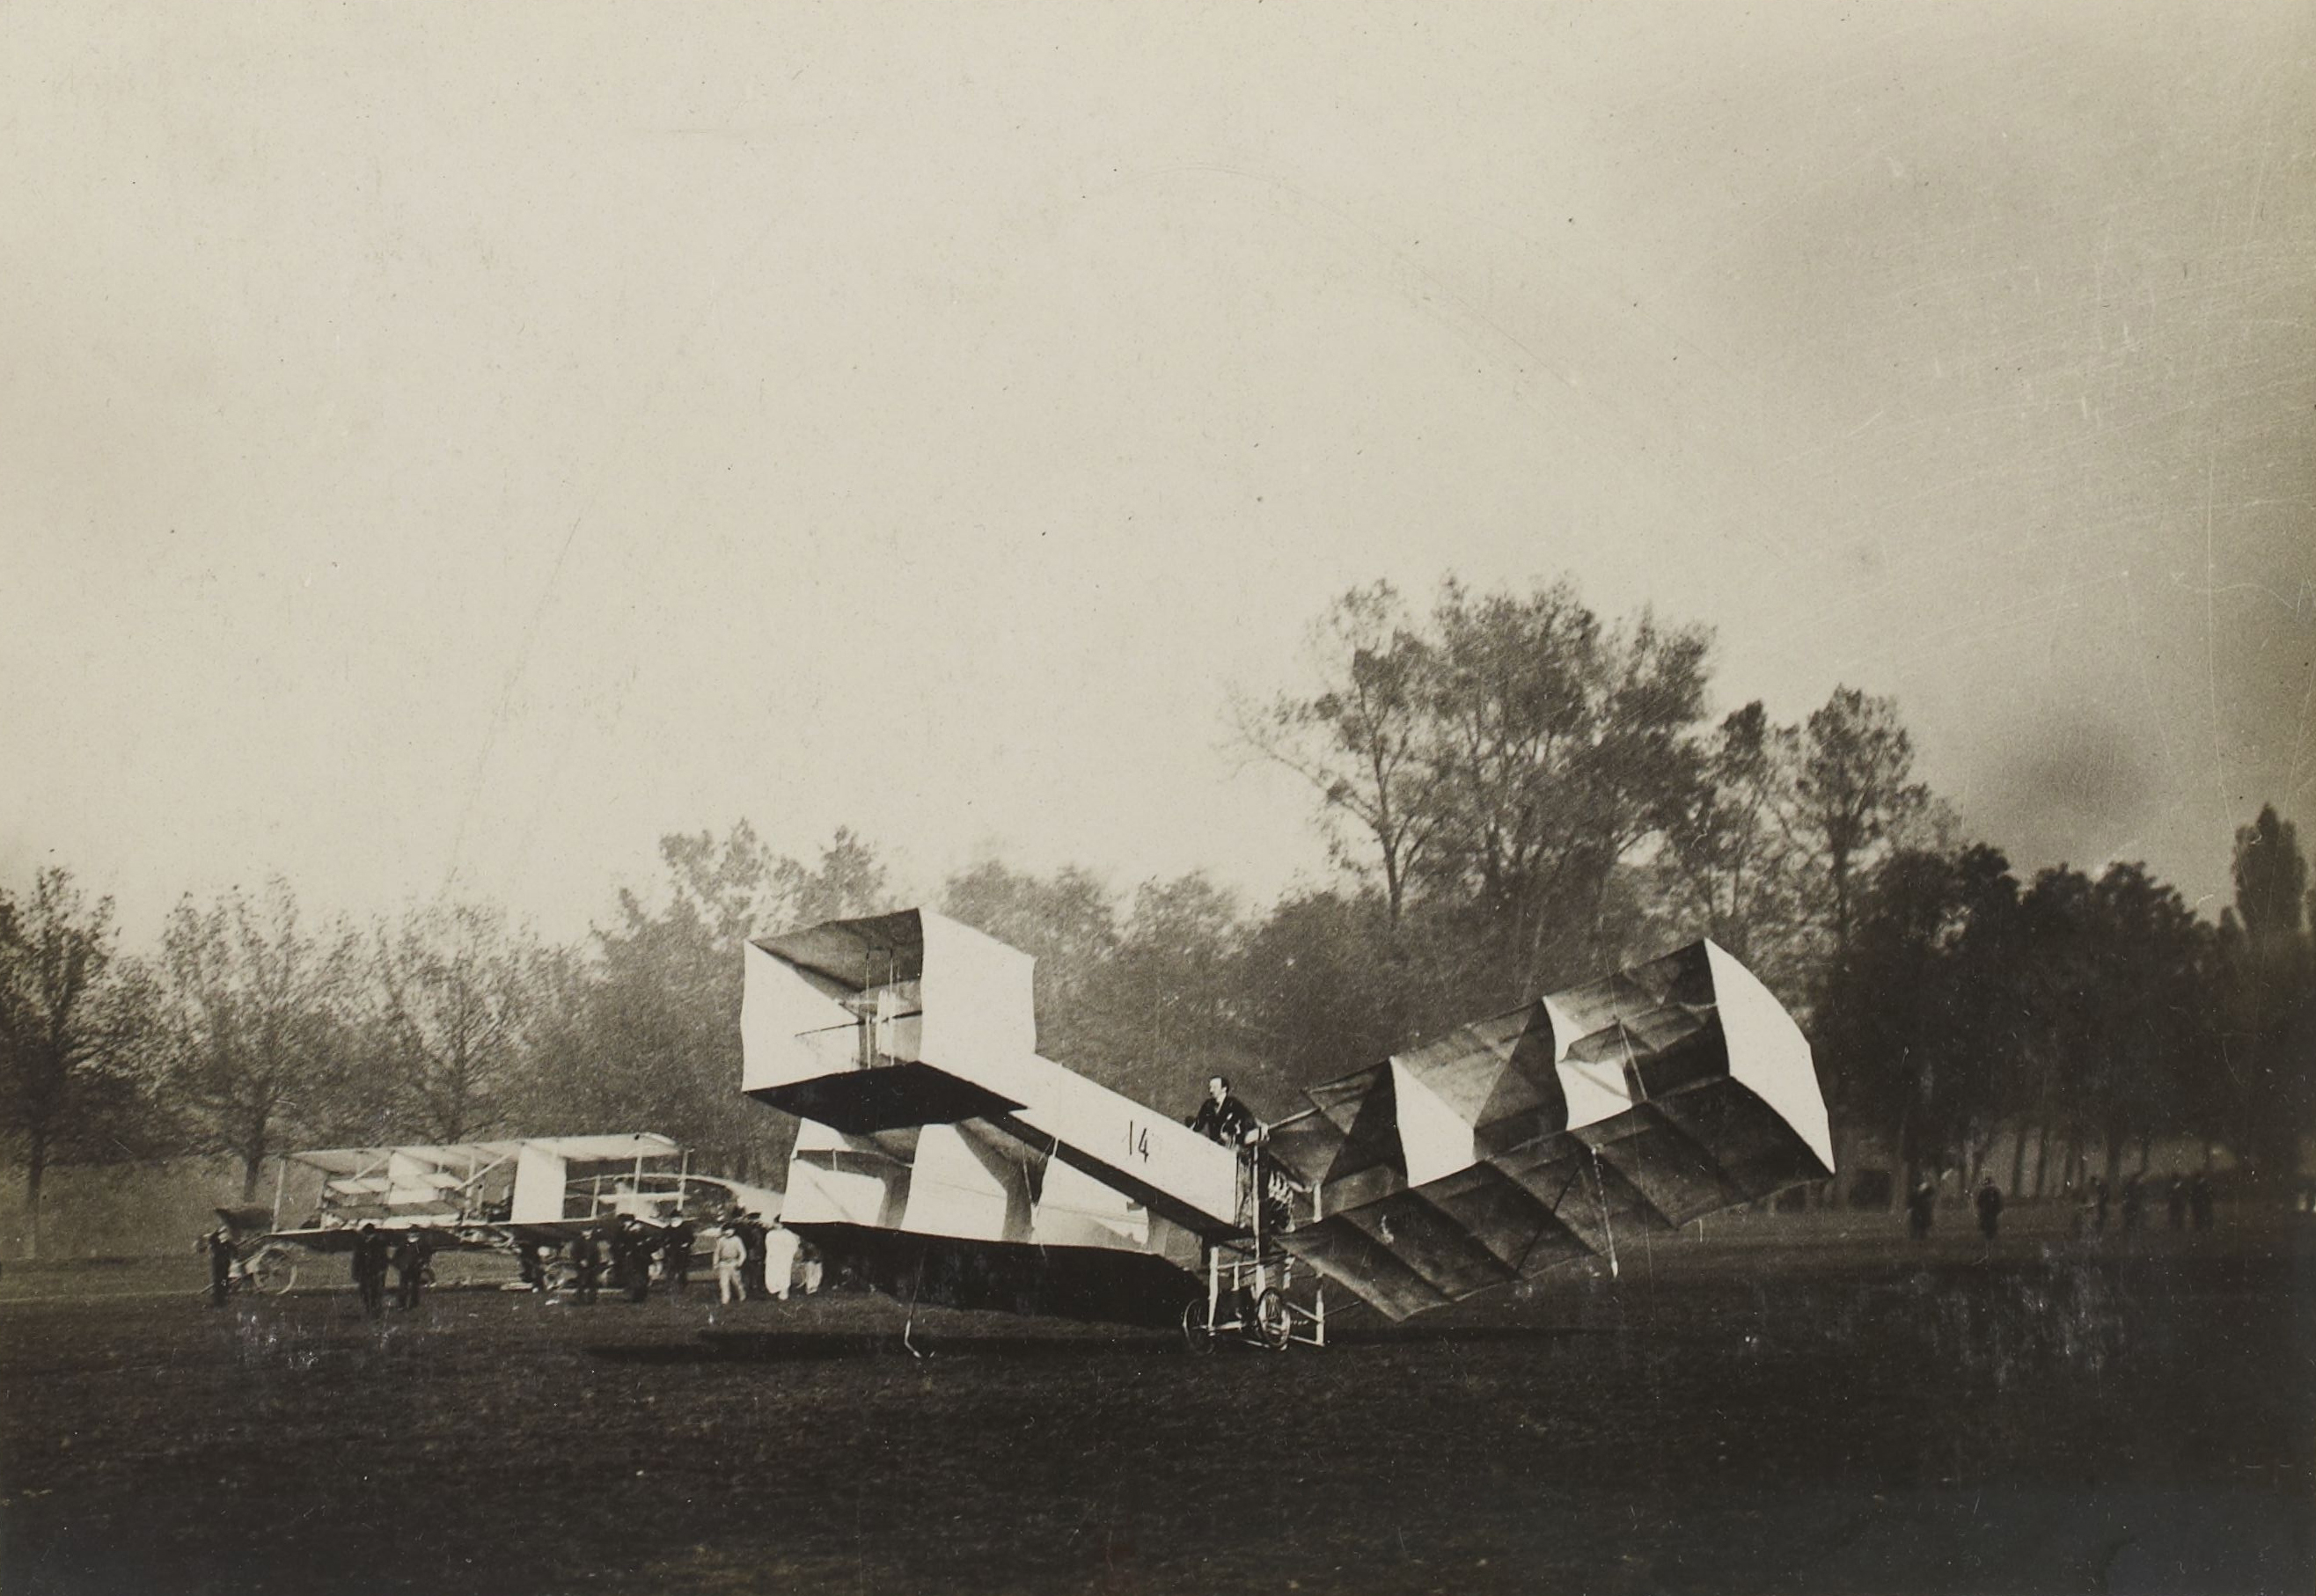
\includegraphics[width=0.55\textwidth, trim={0 0 0 0},clip]{images/14-bis.jpeg}
  \end{center}
  {\footnotesize
  Source: Biblioteca Digital Gallica, id btv1b8433366m, Public Domain, availiable on \citep{Beau1907}\\
  Caption: The 14-bis in its final form, with octagonal-planform interplane ailerons}
    \label{fig:flying_veicle}
\end{figure}
%
Its streamlined shape is optimized for aerodynamic efficiency, minimizing drag and turbulence to facilitate smooth movement through the air. The veicle incorporates pairs of rigid horizontal structures projecting from both sides, designed to provide stability and support during flight \citep{Wipo}, enabling the driver to maintain control even in the presence of strong winds and atmospheric disturbances.\par
%
Within the open cockpit, the driver securely straps into a harness, ready to embark on their mission into lightning storms. The propulsion system powered by the kerosene motor generates the necessary thrust for controlled ascent \citep{Torrens1992}, while the open design ensures an immersive experience for the driver, allowing them to observe and collect data in real-time.\par
%
With its purpose-driven design and reliable motor, the 14-Bis flying vehicle represents an instrumental tool for conducting data collection within lightning storms. The combination of an open cockpit, sturdy structural elements, and efficient propulsion system allows for precise maneuverability and enables researchers to gather valuable insights into the dynamics of these atmospheric phenomena.
%
  \subsection{Electroplumbus Nimbodetector}
%
  The 4th generation Electroplumbus Nimbodetector (figure \ref{fig:electroplumbus}) is a specialized device designed to collect data from a sensor and measure thermal radiation during lightning strikes. The device incorporates a modified version of the Plumbus Combobulator in its core (figure \ref{fig:electroplumbus}a) , along with a specially engineered sensor (figure \ref{fig:electroplumbus}b) that has a prism shape and is filled with an enriched Glowing Schleem substance. The purpose of the device is to gather data on lightning discharges and study their effects on the surrounding air.\par
%
  The sensor within the Electroplumbus Nimbodetector is designed to capture thermal radiation emitted during lightning strikes. When a lightning event occurs, the Glowing Schleem inside the prism-shaped sensor heats up. Due to the low heat capacity of the Schleem, the temperature rise is rapidly measured, providing instant data on the thermal effects of the lightning discharge.\par
%
  To determine the temperature of the air surrounding the sensor, the Plumbus Combobulator within the device incorporates a conventional thermometer with hight heat capaciity. The thermometer is strategically strategically positioned on the rear of the 14-bis flying vehicle to measure the air temperature in the vicinity of the sensor. By comparing the temperature of the Schleem-filled sensor and the air temperature measured by the thermometer, we can establish the temperature difference, which is crucial in assessing the impact of the lightning strikes' radiation on the surrounding air.\par
%
  The Electroplumbus Nimbodetector undergoes rigorous calibration and validation processes to ensure accurate and reliable measurements. Prior to deployment, the device is calibrated against reference instruments and tested under controlled laboratory conditions to establish its performance characteristics. Special attention is given to the sensitivity, precision, and response time of the sensor and thermometer to ensure the accurate capture of data during lightning strikes.
%
\begin{figure}[!h]
  \newcommand\x{0.25}
  \caption{The 4th generation of the Electroplumbus Nimbodetector}
  \begin{center}
    \vspace{-3mm}
    \begin{minipage}[t]{\x\linewidth}
      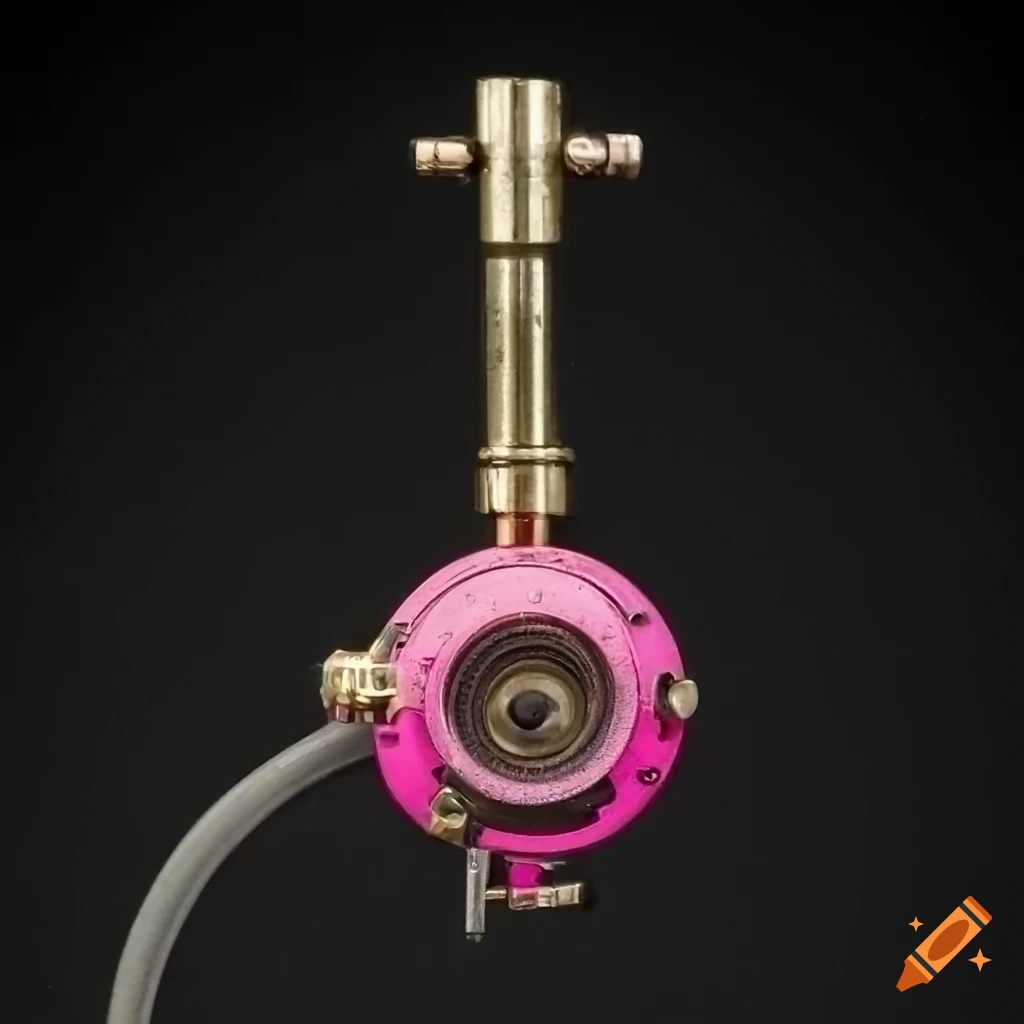
\includegraphics[width = \textwidth, trim={0 0.8cm 0 0.9cm},clip]{images/nimbodetector.png}	
      \captionsetup{justification=centering, font=footnotesize}
      \caption*{(a)}\label{fig:triangle2a}
    \end{minipage}
    \begin{minipage}[t]{\x\linewidth}
      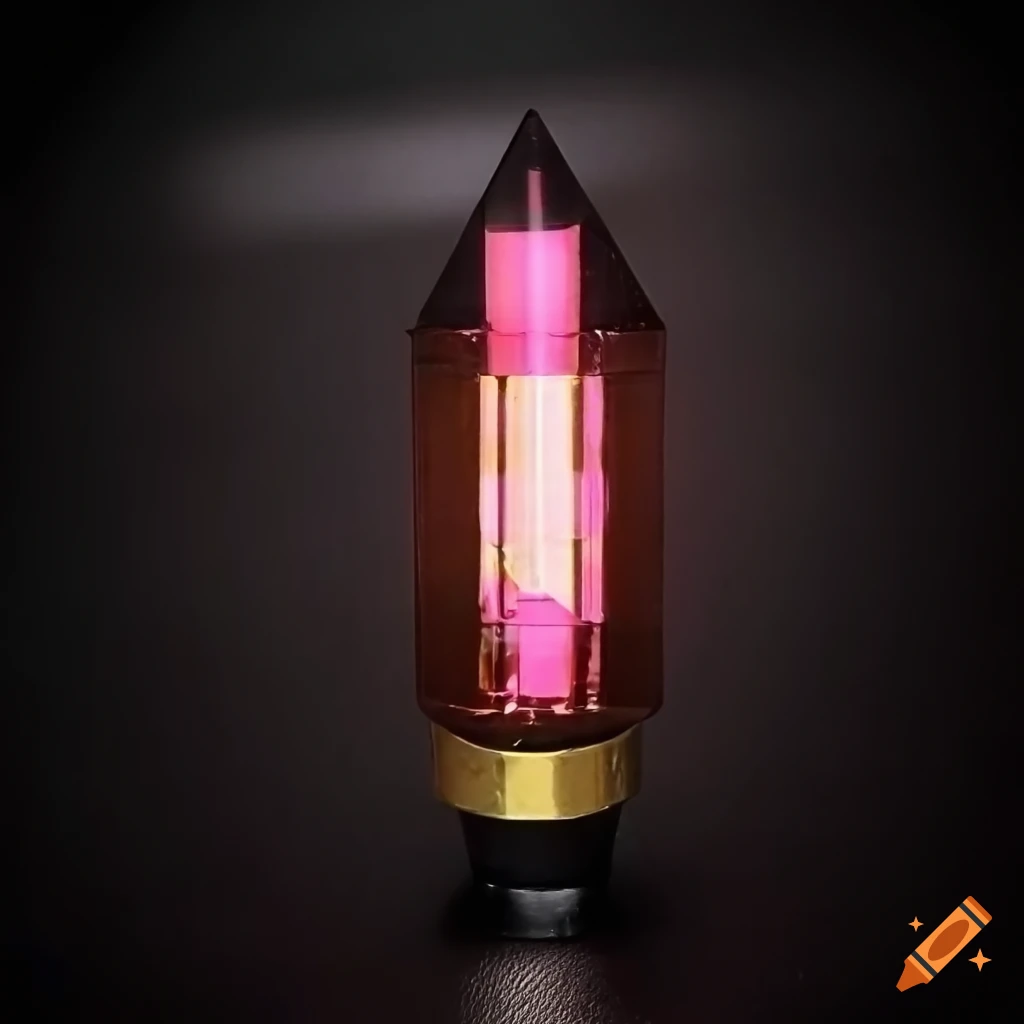
\includegraphics[width = \textwidth, trim={0 0.8cm 0 0.9cm},clip]{images/sensor.png}	
      \captionsetup{justification=centering, font=footnotesize}
      \caption*{(b)}\label{fig:triangle2b}
    \end{minipage}\\
  \end{center}%
  \vspace{-1mm}
  {\footnotesize
  Source: Craiyon website, see \citep{Craiyon}\\
  Caption: The (a) figure displays the core of the device with the Plumbus Combobulator inside and (b) shows the lightning detector filled by enriched Glowing Schleem substance\\
  }
  \label{fig:electroplumbus}
  \end{figure}\vspace{-10mm}
%
\subsection{Data Collection}
%
The data storage component of the Electroplumbus Nimbodetector is an essential element of its operational framework. This system employs a carefully engineered adaptation of the Plumbus Combobulator, which offers fault-tolerant characteristics and efficient data preservation.\par
%
At the core of the data storage mechanism is the utilization of punched tape, designed to withstand various environmental conditions. This robust material ensures the durability and integrity of the captured lightning data, even during adverse weather conditions such as rainfall. The waterproof nature of the tape safeguards the data from moisture, allowing for uninterrupted data collection.\par
%
The adapted Plumbus Combobulator employs a $\SI{0.47}{\micro\meter}$ needle, precisely marking the punched tape as the lightning data is processed. This needle-based mechanism creates a distinct pattern that represents the collected information. With each stroke, a tangible record of the lightning data is imprinted onto the punched tape.\par
%
The tape-based storage medium enables efficient and reliable data preservation. Each $\SI{100}{\milli\meter}$ segment of the punched tape corresponds to a substantial $\SI{1.2E6}{\byte}$ of information. This capacity ensures ample storage space for capturing an extensive volume of lightning data during experiments.\par
%
\section{Data Analysis}
%
\subsection{The Branzine levels}
%
According to the Plumbus Combobulator manufacturer's manual \citep{PlumbusManual}, high levels of Branzine can potentially lead to malfunctions in the Electroplumbus Nimbodetector. Therefore, a preliminary exploratory flight was conducted to investigate the relationship between altitude and Branzine levels.\par
%
During the flight, air samples were gathered at various altitudes to measure the concentration of Branzine, by using the Branzine detector\footnote{Digital Bz897U, available on $^{\circledR}$Airbone Laboratory Instrument Inc.}. The samples were divided into two groups: those collected during rainfall and those obtained under dry conditions. This differentiation aimed to explore any potential impact of precipitation on Branzine levels.
%
The  data was sent to the laboratory, and the results are bellow summarized:
%
\begin{table}[!h]
\caption{Branzine levels}
\vspace{-5mm}
\footnotesize
\begin{center}
  \begin{tabular}{@{}lccc@{}}
  \toprule
                                         & altitude & \multicolumn{2}{c}{Branzine levels {$[ppm]$}} \\ \cmidrule(l){3-4} 
                                         & {$[m]$}  & on rain             & lack of rain            \\ \midrule
  \multirow{8}{*}{\rotatebox[origin=c]{90}{under the clouds} } 
                                         & $100 \pm 1$      & $0.005 \pm 0.001$   &     $0.006 \pm 0.001$  \\
                                         & $200 \pm 1$      & $1.265 \pm 0.001$   &     $1.260 \pm 0.001$  \\
                                         & $500 \pm 1$      & $40.1  \pm 0.1$    &      $40.2 \pm 0.1$   \\
                                         & $1000\pm 1$      & $392   \pm 5$       &      $395  \pm 5$      \\
                                         & $2000\pm 1$      & $609   \pm 5$       &      $607  \pm 5$      \\
                                         & $3000\pm 1$      & $2709  \pm 10$      &     $2701  \pm 10$     \\
                                         & $4000\pm 1$      & $12701 \pm 10$      &     $12699 \pm 10$     \\
                                         & $5000\pm 1$      & $100831 \pm 10$     &     $100827 \pm 10$    \\ \midrule
  \multirow{7}{*}{\rotatebox[origin=c]{90}{above the clouds} }
                                         & $6000\pm 1$       & $-$                &    $280190 \pm 10$                 \\
                                         & $6200\pm 1$       & $-$                &    $518914 \pm 100$                \\ 
                                         & $6400\pm 1$       & $-$                &    $819827 \pm 100$                \\ 
                                         & $6600\pm 1$       & $-$                &    $100827 \pm 100$                \\ 
                                         & $6800\pm 1$       & $-$                &    $1124225 \pm 1000$              \\ 
                                         & $7000\pm 1$       & $-$                &    $6131823 \pm 1000$              \\ 
                                         & $8000\pm 1$       & $-$                &    $9792921 \pm 1000$              \\ \bottomrule
  \end{tabular}\\[3mm]
\end{center}
Caption: The Branzine levels in relation to altitude, over the Atlantic Ocean (August, 1987).\\
\end{table}
\vspace{-6mm}
%
Upon analyzing the data, it was observed that there is a increase in Branzine levels with increasing altitude. However, the rise remained below $0.2\%$, indicating an insignificant effect on the Plumbus performance. These findings align with prior research \citep{Gagaia1923}, which suggests that Branzine levels typically exhibit a notable increase of over $5\%$ in some conditions such as winter seasons or above the Devil's Triangle ($32\%$).
%
\subsection{The radiation levels}
%
Despite the influence of Branzine on the detector, it has been determined that the Electroplumbus Nimbodetector is safe to use under the tested conditions. The Electroplumbus Nimbodetector was successfully installed on the 14-bis flying vehicle, and a series of tests were conducted at altitudes ranging from $\SI{100}{\meter}$ to $\SI{6000}{\meter}$.\par
%
The evaluation began by examining the performance of the Nimbus Detector under heavy rain conditions, comparing the recorded data to measurements obtained in a rainless environment above the clouds. A total of $\SI{12}{\meter}$ of data were collected and recorded on punched tape, with $\SI{30}{\centi\meter}$ obtained in the absence of rain and the remaining length obtained during rainfall.\par
%
After the evaluation, the collected data in the form of punched tape was sent for analysis. The punched tape contained the recorded information obtained by the Nimbus Detector during the data collection. To process and analyze the data, the Monrobot XI computer was used, employing the Foobar Algorithm programmed in FORTRAN (see listing \ref{lst:listing-f90}). The behavior of the sensor can be described by the Stefan-Boltzmann law, which relates the energy radiated by a black body to its temperature.\par
%
According to the Stefan-Boltzmann law, the power radiated by a gray body is proportional to the fourth power of its absolute temperature $T$ and can be expressed as:\par
%
\vspace{-10mm}
\begin{equation}\label{StefanBoltzmannLaw}
  j^{\star}=\sigma T^{4}
\end{equation}
%
\noindent where $j^{\star}$ represents the black-body radiant emittance, and $\sigma$ is the Stefan-Boltzmann constant ($\sigma=5.6704\times10^{-8} Wm^{-2}K^{-4}$).
%
To calculate the heat transfer rate by radiation (almost entire in the infrared spectrum band), we modify the previous equation by incorporating the emissivity $\varepsilon$ of the sensor, to make the sensor behave like a gray body. The modified equation is as follows:
%
\vspace{-5mm}
\begin{equation}
  \frac{Q}{t}=A\sigma\varepsilon (T_{v}^{4} - T_{a}^{4})
\end{equation}
%
Here, $Q \slash t$ represents the radiationheat transfer rate, taking into account the emissivity of the sensor $\varepsilon$ . The emissivity is a dimensionless quantity that varies between $0$ and $1$, where $0$ represents a perfectly reflective surface (no radiation emitted) and $1$ represents a perfectly black body (maximum radiation emitted). In this case, the manufacturer's manual establishes the value $\varepsilon = 0.998$. Also, $A$ is the surface sensor's area ($A=\SI{128.34}{\milli\meter^2}$). $T_v$ and $T_a$ are fuselage and air temperature, respectively.
%
\section{Results and Discussion}
%
The analysis of data collected by the Electroplumbus Nimbodetector reveals a significant correlation between the intensity of lightning strikes and the transfer of thermal radiation. Through a series of field experiments and measurements, we observed a consistent increase in the energy transferred by radiation during lightning events.\par
%
\begin{figure}[!h]
  \caption{Temperature gain as a function of Luminous intensity}
  \vspace{-3mm} 
  \begin{center}
    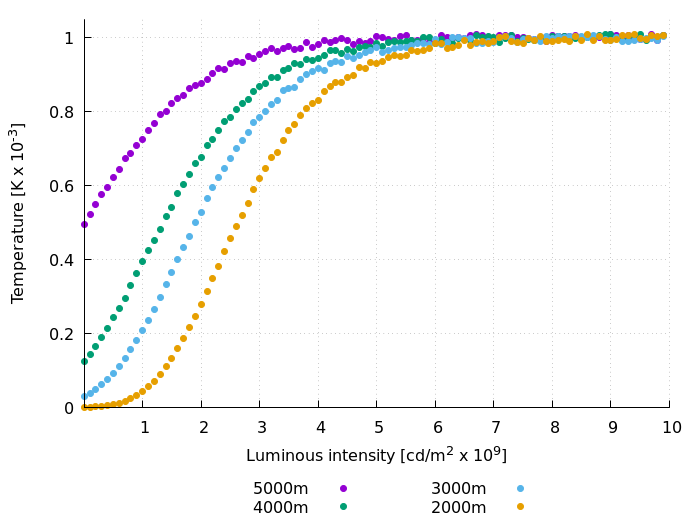
\includegraphics[width=0.85\textwidth, trim={0 0 0 0},clip]{images/graph.png}
  \end{center}
  {\footnotesize Caption: Each set represents an altitude. The graph shows temperature rise as light intensity intensifies on heavy rain}
  \label{fig:graph}
\end{figure}
%
The chart presented in the figure \ref{fig:graph} illustrates the relationship between the intensity of lightning strikes and the corresponding heat transfer rate by radiation. As the intensity of the lightning strike increases, there is a clear upward trend in the energy transferred. This observation supports the hypothesis that lightning strikes contribute to an enhanced transfer of thermal radiation to the surrounding air.\par
%
The strong correlation observed between lightning strikes and the energy transferred by radiation reinforces the reliability of the data collected by the Electroplumbus Nimbodetector. These findings provide valuable insights into the thermal dynamics associated with lightning discharges and contribute to a better understanding of the effects of lightning on the surrounding environment.\par
%
Moreover, it is important to note that light alone cannot directly heat gas molecules. Instead, during a lightning strike, the light emitted excites the electrons in atoms within the detector. These atoms are already vibrating at a certain frequency. Some of these atoms vibrate with sufficient vigor that their vibrational energy matches the electronic energy (photons) absorbed from the lightning, effectively reaching resonance with the solar energy. As a result, these atoms undergo a quantum transition from being ``electronically excited" to ``vibrationally excited", causing the entire atom to move. The surrounding air perceives this excited vibration as ``heat."\par
%
This mechanism provides a deeper understanding of how the energy from a lightning strike is converted into thermal energy in the air. By studying the vibrational and electronic transitions occurring within the atoms of the detector, we can further elucidate the intricate processes involved in the thermal effects of lightning discharges.\par
%
In conclusion, this study demonstrates a strong correlation between the intensity of lightning strikes and the transfer of thermal radiation. The data collected by the Electroplumbus Nimbodetector, along with the presented chart, provides robust evidence supporting this relationship. Additionally, the exploration of the underlying processes involving electronic and vibrational transitions within the detector atoms enhances our comprehension of how lightning energy is converted into heat in the surrounding air. These findings contribute to the scientific understanding of lightning-induced thermal phenomena and lay the foundation for future research in this field.
%
\section*{Acknowledgements}
%
We gratefully acknowledge the Lupus Institute for their financial support, which has made this work possible. Also, we want to express our sincere appreciation to the open.ai for its invaluable assistance in the development of this fictional scientific paper.
%
\bibliography{references}
%
\theauthorcontributions
%
\howtocite
%
\section*{Appendix}
%
\raggedleft\setstretch{1.0}\noindent
\begin{minipage}[b]{\linewidth-6.5mm}
  \lstinputlisting[caption=Foobar source code, label={lst:listing-f90}, language=Fortran]{foobar.f90}
\end{minipage}
%
\end{document}
